\documentclass[11pt]{beamer}
\usetheme{Rochester}
\usepackage[utf8]{inputenc}
\usepackage{amsmath}
\usepackage{amsfonts}
\usepackage{amssymb}
\usepackage{graphicx}
%\author{}
%\title{}
%\setbeamercovered{transparent} 
%\setbeamertemplate{navigation symbols}{} 
%\logo{} 
%\institute{} 
%\date{} 
%\subject{} 
\begin{document}

\begin{frame}
\title{Computational Astrophysics}
\author{E. Larrañaga}
\institute{Observatorio Astronómico Nacional\\
Universidad Nacional de Colombia}
\titlepage
\end{frame}

\begin{frame}{Outline}
\tableofcontents
\end{frame}

\section{2 Dimensional Advection}
\begin{frame}[fragile]{2 Dimensional Advection}
The two-dimensional linear advection equation is
\begin{equation}
\partial_t a + u \partial_x a + v \partial_y a = 0
\label{eq:advect2d}
\end{equation}
where $u$ is the velocity in the $x$-direction and $v$ is the velocity in
the $y$-direction.  
\bigskip

We denote the average of $a(x,y,t)$ in a zone $i,j$ as
$a_{i,j}$.  Here, $i$ is the index in the $x$-direction and $j$ is the
index in the $y$-direction.
\bigskip 

As in the one-dimensional case, we will extend the domain with a
perimeter of ghost cells to set the boundary conditions.
\end{frame}

\begin{frame}[fragile]{2 Dimensional Grid}
\begin{center}
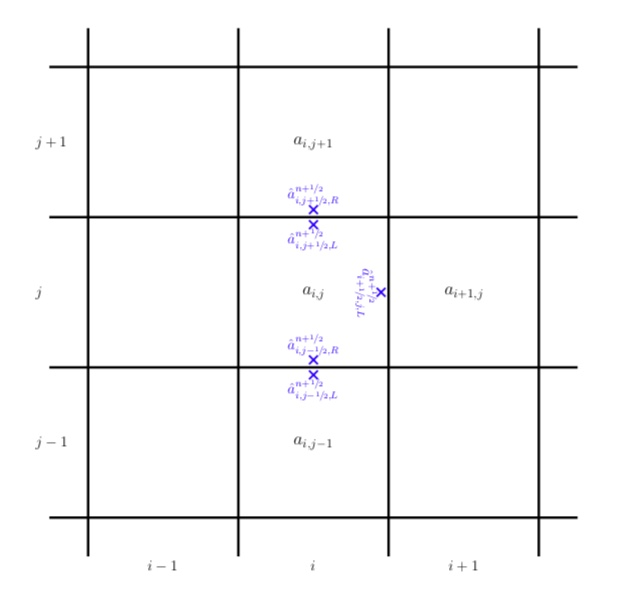
\includegraphics[scale=0.3]{2DGrid}
\end{center}
\end{frame}


\begin{frame}[fragile]{2 Dimensional Advection}
Since $u$ and $v$ are constant, we can
move them inside the derivatives,
\begin{equation}
\partial_t a + \partial_x (u a) + \partial_y (v a) = 0.
\end{equation}

We 
define the average of $a$ in a zone by integrating it over the
volume:
\begin{equation}
a_{i,j} = \frac{1}{\Delta x \Delta y} 
   \int_{x_{i-\frac{1}{2}}}^{x_{i+\frac{1}{2}}} \int_{y_{j-\frac{1}{2}}}^{y_{j+\frac{1}{2}}} 
   a(x,y,t) \, dx \, dy
\end{equation}
\end{frame}

\begin{frame}[fragile]{2 Dimensional Advection}
Integrating the advection equation over $x$ and $y$, we obtain
\begin{align}
\frac{1}{\Delta x \Delta y} 
  \int_{x_{i-\frac{1}{2}}}^{x_{i+\frac{1}{2}}} 
  \int_{y_{j-\frac{1}{2}}}^{y_{j+\frac{1}{2}}} a_t \, dx \, dy =  
  &- \frac{1}{\Delta x \Delta y}
       \int_{x_{i-\frac{1}{2}}}^{x_{i+\frac{1}{2}}} \int_{y_{j-\frac{1}{2}}}^{y_{j+\frac{1}{2}}}
      (u a)_x \, dx \, dy \nonumber \\
  &- \frac{1}{\Delta x \Delta y}
       \int_{x_{i-\frac{1}{2}}}^{x_{i+\frac{1}{2}}} \int_{y_{j-\frac{1}{2}}}^{y_{j+\frac{1}{2}}}
      (v a)_y \, dx \, dy 
\end{align}
\end{frame}

\begin{frame}[fragile]{2 Dimensional Advection}
Integration in the left hand side gives
\begin{align}
 \frac{\partial a_{i,j}}{\partial t} =
  &- \frac{1}{\Delta x\Delta y} \int_{y_{j-\frac{1}{2}}}^{y_{j+\frac{1}{2}}}
     \left \{ (u a)_{i+\frac{1}{2},j} - (u a)_{i-\frac{1}{2},j} \right \} dy \nonumber \\
  &- \frac{1}{\Delta x\Delta y} \int_{x_{i-\frac{1}{2}}}^{x_{i+\frac{1}{2}}}
     \left \{ (v a)_{i,j+\frac{1}{2}} - (v a)_{i,j-\frac{1}{2}} \right \} dx
\end{align}
\end{frame}

\begin{frame}[fragile]{2 Dimensional Advection}
and integrating with respect to time 
\begin{align}
 a_{i,j}^{n+1} - a_{i,j}^n = 
  &- \frac{1}{\Delta x\Delta y} \int_{t^n}^{t^{n+1}} \int_{y_{j-\frac{1}{2}}}^{y_{j+\frac{1}{2}}}
     \left \{ (u a)_{i+\frac{1}{2},j} - (u a)_{i-\frac{1}{2},j} \right \} dy dt \nonumber \\
  &- \frac{1}{\Delta x\Delta y} \int_{t^n}^{t^{n+1}} \int_{x_{i-\frac{1}{2}}}^{x_{i+\frac{1}{2}}}
     \left \{ (v a)_{i,j+\frac{1}{2}} - (v a)_{i,j-\frac{1}{2}} \right \} dx dt
\end{align}
\end{frame}

\begin{frame}[fragile]{2 Dimensional Advection}
We define the flux through the interface as the average over the face
of that interface and time, 
\begin{itemize}
\item x-face:
\begin{equation}
\langle (ua)_{i+\frac{1}{2},j}\rangle_{(t)} = \frac{1}{\Delta y \Delta t}
    \int_{t^n}^{t^{n+1}} \int_{y_{j-\frac{1}{2}}}^{y_{j+\frac{1}{2}}} (ua)_{i+\frac{1}{2},j}\, dy dt
\end{equation}
\item y-face
\begin{equation}
\langle (va)_{i,j+\frac{1}{2}}\rangle_{(t)} = \frac{1}{\Delta x \Delta t}
    \int_{t^n}^{t^{n+1}} \int_{x_{i-\frac{1}{2}}}^{x_{i+\frac{1}{2}}} (va)_{i,j+\frac{1}{2}}\, dx dt 
\end{equation}
\end{itemize}
where $\langle . \rangle_{(t)}$ denotes the time-average over the face.
\end{frame}

\begin{frame}[fragile]{2 Dimensional Advection}
Now, we replace the average in
time with the flux at the midpoint in time and the average over the face
with the flux at the center of the face,
\begin{equation}
\langle (ua)_{i+\frac{1}{2},j} \rangle_{(t)} \approx (ua)_{i+\frac{1}{2},j}^{n+\frac{1}{2}}
\end{equation}
\end{frame}

\begin{frame}[fragile]{2 Dimensional Advection}
Then, 
\begin{equation}
a_{i,j}^{n+1} = a_{i,j}^n - \Delta t \left [
   \frac{(ua)_{i+\frac{1}{2},j}^{n+\frac{1}{2}} - (ua)_{i-\frac{1}{2},j}^{n+\frac{1}{2}}}{\Delta x} +
   \frac{(va)_{i,j+\frac{1}{2}}^{n+\frac{1}{2}} - (va)_{i,j-\frac{1}{2}}^{n+\frac{1}{2}}}{\Delta y} \right ]
\end{equation}
\end{frame}

\begin{frame}[fragile]{Dimensionally split method}
In a split method, we update the state in each coordinate direction
independently.  We will consider the {\em Strang splitting}, where we alternate
the order of the dimensional updates each timestep.  An update through
$\Delta t$ consists of $x$ and $y$ sweeps and appears as
\begin{eqnarray}
 \frac{a_{i,j}^\star - a_{i,j}^n}{\Delta t} &=&
  - \frac{ u a_{i+\frac{1}{2},j}^{n+\frac{1}{2}} - u a_{i-\frac{1}{2},j}^{n+\frac{1}{2}} }{\Delta x} \label{eq:splitx}\\
 \frac{a_{i,j}^{n+1} - a_{i,j}^\star}{\Delta t} &=&
  - \frac{ v a_{i,j+\frac{1}{2}}^{\star,n+\frac{1}{2}} - v a_{i,j-\frac{1}{2}}^{\star,n+\frac{1}{2}} }{\Delta y} \label{eq:splity}
\end{eqnarray}
\end{frame}

\begin{frame}[fragile]{Dimensionally split method}
The states
$a_{i+\frac{1}{2},j}^{n+\frac{1}{2}}$ are calculated as
\begin{eqnarray}
a_{i+\frac{1}{2},j}^{n+\frac{1}{2}} &=& a_{i,j}^n + 
  \frac{\Delta x}{2} \left .\frac{\partial a}{\partial x} \right |_{i,j} + 
  \frac{\Delta t}{2} \left .\frac{\partial a}{\partial t} \right |_{i,j} + 
  \mathcal{O}(\Delta x^2) + \mathcal{O}(\Delta t^2) \nonumber \\
 &=& a_{i,j}^n + 
   \frac{\Delta x}{2} \left .\frac{\partial a}{\partial x} \right |_{i,j} + 
   \frac{\Delta t}{2} \left ( 
   - u \left .\frac{\partial a}{\partial x} \right |_{i,j} \right
   ) + \ldots \nonumber \\
    &=& a_{i,j}^n + 
   \frac{\Delta x}{2} \left ( 1 - \frac{\Delta t}{\Delta x} u \right ) 
   \left .\frac{\partial a}{\partial x} \right |_{i,j} +
   \ldots \label{eq:statels}
\end{eqnarray}
\end{frame}

\begin{frame}[fragile]{2 Dimensional Grid}
\begin{center}
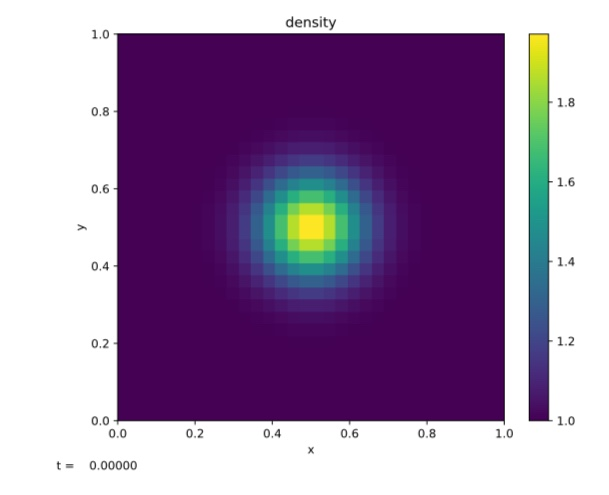
\includegraphics[scale=0.3]{Gaussian}
\end{center}
\end{frame}

\begin{frame}[fragile]{2 Dimensional Grid}
\begin{center}
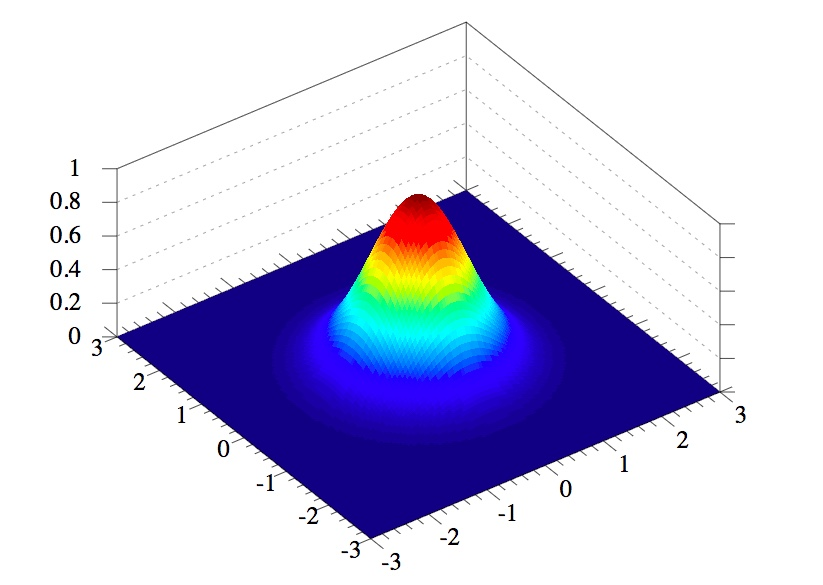
\includegraphics[scale=0.3]{Gaussian2}
\end{center}
\end{frame}

\begin{frame}[fragile]{Next Class}
\end{frame}

\end{document}
